% !TEX program = xelatex
% !TEX TS-program = xelatex
% =============================================================================
% Compile with XeLaTeX (needed for Helvetica Neue):  xelatex presentation.tex
% Style: Swiss / editorial grid. Label column left, content column right,
% hairline rules, regular-weight Helvetica, monochrome, minimal text.
% =============================================================================
\documentclass[aspectratio=169, 10pt]{beamer}

% -----------------------------------------------------------------------------
% Fonts (compatible with both pdfLaTeX and XeLaTeX/LuaLaTeX)
% -----------------------------------------------------------------------------
\usepackage{iftex}
\ifPDFTeX
  \newcommand{\timesfont}{\rmfamily}
  \newcommand{\tighttimes}{\rmfamily\itshape}
  \usepackage[utf8]{inputenc}
  \usepackage[T1]{fontenc}
  % Helvetica if installed (sudo tlmgr install helvetic), otherwise Latin Modern
  \IfFileExists{uhvr8t.tfm}{\usepackage[scaled]{helvet}}{\usepackage{lmodern}}
  \renewcommand{\familydefault}{\sfdefault}
\else
  \usefonttheme{professionalfonts}
  \usepackage{fontspec}
  \setsansfont{Helvetica Neue}
  \setmainfont{Helvetica Neue}
  \newfontfamily\timesfont{Times New Roman}
  \newcommand{\tighttimes}{\timesfont\itshape\addfontfeatures{LetterSpace=-6}}
  \renewcommand{\familydefault}{\sfdefault}
\fi

\usepackage{tikz}
\usepackage{tcolorbox}
\tcbuselibrary{skins}
\usetikzlibrary{arrows.meta, calc}
\newcommand{\nohyph}{\hyphenpenalty 10000 \exhyphenpenalty 10000 }

% -----------------------------------------------------------------------------
% Palette (monochrome)
% -----------------------------------------------------------------------------
\definecolor{ink}{RGB}{17, 17, 17}
\definecolor{mute}{RGB}{120, 120, 120}
\definecolor{numgray}{RGB}{185, 185, 185}
\definecolor{hair}{RGB}{170, 170, 170}
\definecolor{bggray}{RGB}{228, 228, 228}
\definecolor{panel}{RGB}{240, 240, 240}
\definecolor{accent}{RGB}{255, 79, 0}
\definecolor{uireal}{RGB}{30,127,60}
\definecolor{uienh}{RGB}{154,91,0}
\definecolor{uigen}{RGB}{91,60,196}
\definecolor{uiunk}{RGB}{85,85,91}

% -----------------------------------------------------------------------------
% Grid: page 16cm x 9cm
%   outer margin 0.6cm | label column 0.6-4cm | content column 4.6-15.4cm
% -----------------------------------------------------------------------------
\setbeamertemplate{navigation symbols}{}
\setbeamercolor{background canvas}{bg=white}
\setbeamercolor{normal text}{fg=ink}
\setbeamersize{text margin left=3.2cm, text margin right=0.6cm}

% -----------------------------------------------------------------------------
% Type
% -----------------------------------------------------------------------------
\newcommand{\metafont}{\fontsize{5.5pt}{7pt}\selectfont}
\newcommand{\meta}[1]{{\metafont #1}}
\newcommand{\bodysm}[1]{{\fontsize{8pt}{11pt}\selectfont\raggedright #1\par}}
\newcommand{\display}[1]{{\fontsize{20pt}{22pt}\selectfont #1\par}}
\newcommand{\subhead}[1]{{\fontsize{10pt}{12pt}\selectfont #1\par}\vspace{0.15cm}}

% Hairline + small heading above a column
\newcommand{\colrule}[1]{{\color{hair}\rule{\linewidth}{0.4pt}}\par\vspace{0.12cm}\subhead{#1}}

% Row with gray label: \entry{O1}{text}
\newcommand{\entry}[2]{%
  \noindent\makebox[0.95cm][l]{\fontsize{8pt}{11pt}\selectfont\color{mute}#1}%
  \parbox[t]{\dimexpr\linewidth-0.95cm}{\fontsize{8pt}{11pt}\selectfont\raggedright #2}\par\vspace{0.1cm}}

% Large list row with light-gray number: \listrow{1}{text}
\newcommand{\listrow}[2]{{\fontsize{17pt}{21pt}\selectfont\noindent\makebox[0.9cm][l]{\color{numgray}#1}\parbox[t]{\dimexpr\linewidth-0.9cm}{\raggedright #2}\par}}

% Objective / research question row: \rqrow{n}{objective}{question}
\newcommand{\rqrow}[3]{%
  \par\vspace{0.07cm}{\color{hair}\hrule height 0.3pt}\vspace{0.1cm}
  \noindent\makebox[0.6cm][l]{\fontsize{9pt}{12pt}\selectfont\color{numgray}#1}%
  \parbox[t]{3.4cm}{\fontsize{9pt}{12pt}\selectfont\raggedright #2}%
  \parbox[t]{\dimexpr\linewidth-4cm}{\fontsize{9pt}{12pt}\selectfont\raggedright #3}\par\vspace{0.05cm}}

% Row with data-source column: \rqrowm{n}{objective}{question}{source}
\newcommand{\rqrowm}[4]{%
  \par\vspace{0.07cm}{\color{hair}\hrule height 0.3pt}\vspace{0.09cm}
  \noindent\makebox[0.55cm][l]{\fontsize{8pt}{11pt}\selectfont\color{numgray}#1}%
  \parbox[t]{2.65cm}{\fontsize{8pt}{11pt}\selectfont\raggedright #2}%
  \parbox[t]{5.0cm}{\fontsize{8pt}{11pt}\selectfont\raggedright #3}%
  \hspace{0.25cm}\parbox[t]{\dimexpr\linewidth-8.45cm}{\fontsize{8pt}{11pt}\selectfont\raggedright\leavevmode\color{mute}#4}\par\vspace{0.04cm}}

% Compact dash bullet
\newcommand{\bul}[1]{\noindent\makebox[0.3cm][l]{\fontsize{8pt}{11pt}\selectfont\color{mute}--}\parbox[t]{\dimexpr\linewidth-0.3cm}{\fontsize{8pt}{11pt}\selectfont\raggedright #1}\par\vspace{0.06cm}}

% Finding row: \fdrow{n}{RQ}{finding}{evidence}
\newcommand{\fdrow}[4]{%
  \par\vspace{0.07cm}{\color{hair}\hrule height 0.3pt}\vspace{0.1cm}
  \noindent\makebox[0.55cm][l]{\fontsize{8pt}{10.5pt}\selectfont\color{numgray}#1}%
  \parbox[t]{2.3cm}{\fontsize{8pt}{10.5pt}\selectfont\raggedright #2}%
  \parbox[t]{4.75cm}{\fontsize{8pt}{10.5pt}\selectfont\raggedright #3}%
  \hspace{0.2cm}\parbox[t]{\dimexpr\linewidth-7.8cm}{\fontsize{8pt}{10.5pt}\selectfont\raggedright #4}\par\vspace{0.05cm}}

% Desk research row: \deskrow{source}{key point}
\newcommand{\deskrow}[2]{%
  \par\vspace{0.07cm}{\color{hair}\hrule height 0.3pt}\vspace{0.1cm}
  \noindent\parbox[t]{3.6cm}{\fontsize{8.5pt}{11pt}\selectfont\raggedright #1}%
  \parbox[t]{\dimexpr\linewidth-3.6cm}{\fontsize{8.5pt}{11pt}\selectfont\raggedright #2}\par\vspace{0.04cm}}

% 5W1H row: \wrow{label}{text}
\newcommand{\wrow}[2]{%
  \par\vspace{0.06cm}{\color{hair}\hrule height 0.3pt}\vspace{0.1cm}
  \noindent\parbox[t]{1.6cm}{\fontsize{9pt}{12pt}\selectfont\leavevmode\color{mute}#1}%
  \parbox[t]{\dimexpr\linewidth-1.6cm}{\fontsize{9pt}{12pt}\selectfont\raggedright #2}\par\vspace{0.03cm}}

% Big stat tile: \stat{number}{caption}
\newcommand{\stat}[2]{{\color{hair}\rule{\linewidth}{0.4pt}}\par\vspace{0.1cm}{\fontsize{22pt}{24pt}\selectfont #1\par}\vspace{0.08cm}{\fontsize{8pt}{10.5pt}\selectfont\raggedright\color{mute}#2\par}}
% Body text at 9pt
\newcommand{\pbody}[1]{{\fontsize{9pt}{12pt}\selectfont\raggedright #1\par}}

% Idea row: \idea{n}{idea}{reason}{chosen 1/0}
\newcommand{\idea}[4]{%
  \noindent\makebox[0.45cm][l]{\fontsize{8.5pt}{11pt}\selectfont\color{numgray}#1}%
  \parbox[t]{\dimexpr\linewidth-0.45cm}{\fontsize{8.5pt}{11pt}\selectfont\raggedright\ifnum#4=1 \textbf{#2}\else #2\fi\\[-0.02cm]{\fontsize{7.5pt}{9.5pt}\selectfont\ifnum#4=1 \color{accent}\else\color{mute}\fi #3}}\par\vspace{0.07cm}}

% Edge case block: \edgecase{title}{how it is handled}{status}
\newcommand{\edgecase}[3]{\colrule{#1}{\fontsize{8pt}{10.5pt}\selectfont\raggedright #2\par}\vspace{0.06cm}{\fontsize{7pt}{9pt}\selectfont\color{accent}#3\par}\vspace{0.22cm}}

% Final UI label: \uilabel{colourkey}{text}
\newcommand{\uilabel}[2]{{\fontsize{8pt}{10pt}\selectfont\bfseries\color{ui#1}#2\par}}
% Trust row: \trustrow{n}{title}{text}
\newcommand{\trustrow}[3]{\par\vspace{0.05cm}{\color{hair}\hrule height 0.3pt}\vspace{0.1cm}\noindent\makebox[0.5cm][l]{\raisebox{-0.02cm}{\tikz\node[circle, fill=accent, text=white, inner sep=0, minimum size=0.36cm, font=\fontsize{7.5pt}{8pt}\selectfont\bfseries]{#1};}}\parbox[t]{\dimexpr\linewidth-0.5cm}{\raggedright\hyphenpenalty 10000 \fontsize{9pt}{11.5pt}\selectfont\textbf{#2}\\{\fontsize{8pt}{10.5pt}\selectfont\color{mute}#3}}\par\vspace{0.03cm}}
% Wireframe caption: \wfnote{n}{title}{evolution}
\newcommand{\wfnote}[3]{\raggedright{\fontsize{9pt}{11pt}\selectfont{\color{numgray}#1}\enspace\textbf{#2}\par}\vspace{0.04cm}{\fontsize{8pt}{10.5pt}\selectfont\color{mute}#3\par}}

% Empty panel to fill in later: \blank{height}
\newcommand{\blank}[1]{\begin{tcolorbox}[enhanced, colback=panel, frame hidden, arc=0mm, height=#1, boxsep=0pt, left=0pt, right=0pt, top=0pt, bottom=0pt]\mbox{}\end{tcolorbox}}

% -----------------------------------------------------------------------------
% Page chrome: \chrome{section label}{right meta}
% -----------------------------------------------------------------------------
\newcommand{\chromeL}{}
\newcommand{\chromeR}{}
\newcommand{\chromeLC}{hair}
\newcommand{\chrome}[2]{\gdef\chromeL{#1}\gdef\chromeR{#2}\gdef\chromeLC{hair}\leavevmode\par}
% Same, for orange slides: black top line
\newcommand{\chromeorange}[2]{\gdef\chromeL{#1}\gdef\chromeR{#2}\gdef\chromeLC{ink}\leavevmode\par}
% Drawn as the slide background, so it appears on every single compile
\setbeamertemplate{background}{%
  \begin{tikzpicture}
    \useasboundingbox (0,0) rectangle (\paperwidth,\paperheight);
    \fill[ink] (0.72cm, \paperheight-0.42cm) circle (0.12cm);
    \fill[ink] (0.72cm, \paperheight-0.70cm) circle (0.12cm);
    \draw[\chromeLC, line width=0.4pt] (0.6cm, \paperheight-1.0cm) -- (\paperwidth-0.6cm, \paperheight-1.0cm);
    \node[anchor=north west, inner sep=0, align=left, font=\metafont] at (0.6cm, \paperheight-1.15cm) {\chromeL};
    \node[anchor=north east, inner sep=0, align=right, font=\metafont] at (\paperwidth-0.6cm, \paperheight-0.38cm) {\chromeR};
    \node[anchor=south east, inner sep=0, font=\metafont] at (\paperwidth-0.6cm, 0.3cm) {\insertframenumber\ / \inserttotalframenumber};
    \draw[ink, line width=1.6pt] (0.3cm, 0.25cm) -- (0.3cm, 4.2cm);
    \draw[ink, line width=1.6pt] (\paperwidth-0.3cm, 0.25cm) -- (\paperwidth-0.3cm, 4.2cm);
  \end{tikzpicture}%
}

% Standard slide opening: title area
\newcommand{\slidehead}[1]{\vspace*{0.85cm}\display{#1}\vspace{0.3cm}}

% Chapter opener: orange background, big number, title
\newcommand{\chapterslide}[2]{%
{\setbeamercolor{background canvas}{bg=accent}
\begin{frame}[plain, t]
  \chromeorange{}{}
  \vspace*{1.15cm}
  \hfill{\fontsize{80pt}{80pt}\selectfont #1}\par
  \vfill
  {\fontsize{40pt}{40pt}\selectfont\tighttimes #2\par}
  \vspace{0.75cm}
\end{frame}}}

\begin{document}

% =============================================================================
% COVER (orange)
% =============================================================================
{\setbeamercolor{background canvas}{bg=accent}
\begin{frame}[plain, t]
  \chromeorange{Product Design\\Intern Challenge}{NOVEMBER 2026}

  \vspace*{0.85cm}
  {\fontsize{30pt}{31pt}\selectfont Real, AI-enhanced\\or AI-generated?\par}

  \vfill
  {\color{ink}\rule{\linewidth}{0.4pt}}\par\vspace{0.12cm}
  \begin{columns}[T, onlytextwidth]
    \begin{column}{0.32\linewidth}\meta{\color{ink}Candidate}\\[0.05cm]\bodysm{Bulluraj Mutum\\[0.05cm]M.Des (UX)}\end{column}
    \begin{column}{0.32\linewidth}\meta{\color{ink}Role}\\[0.05cm]\bodysm{Product Design Intern}\end{column}
    \begin{column}{0.32\linewidth}\meta{\color{ink}Brief}\\[0.05cm]\bodysm{UI/UX design challenge}\end{column}
  \end{columns}
  \vspace{0.75cm}
\end{frame}
}

% =============================================================================
% CONTENTS
% =============================================================================
\begin{frame}[plain, t]
  \chrome{Contents}{}

  \vfill
  \listrow{1}{Problem}
  \listrow{2}{Concept}
  \listrow{3}{Flow}
  \listrow{4}{Design}
  \listrow{5}{Prototype}
  \listrow{6}{Measure}
  \vspace{0.7cm}
\end{frame}

% =============================================================================
% 01 PROBLEM
% =============================================================================
\chapterslide{01}{Problem}

\begin{frame}[plain, t]
  \chrome{1\quad Problem}{PROBLEM UNDERSTANDING}

  \slidehead{Problem understanding}
  {\fontsize{13pt}{16pt}\selectfont People can't reliably tell real from AI, and feeling sure is a weak guide.\par}
  \vspace{0.35cm}
  \begin{columns}[T, onlytextwidth]
    \begin{column}{0.235\linewidth}\stat{58\%}{right overall; guessing is 50\%}\end{column}
    \begin{column}{0.235\linewidth}\stat{44\%}{spotted the AI edit on a real photo (pair 1)}\end{column}
    \begin{column}{0.235\linewidth}\stat{5/20}{wrong answers rated ``very sure'' (4--5)}\end{column}
    \begin{column}{0.235\linewidth}\stat{2 vs 0}{would trust a friend's image vs a stranger's}\end{column}
  \end{columns}
  \vspace{0.35cm}
  \bodysm{{\color{mute}What shaped the direction:} people judge by gut (``light'', ``sharpness'', ``instinct''), no single check is reliable, and friends' images get the least scrutiny.}
  \meta{\color{mute}From my research: survey of 16 people (18--35) and desk research. (from the User Research Assignment)}
\end{frame}

\begin{frame}[plain, t]
  \chrome{1\quad Problem}{TARGET USER \& USE CASE}

  \slidehead{Target user \& use case}
  \begin{columns}[T, onlytextwidth]
    \begin{column}{0.31\linewidth}\colrule{Who}
      \pbody{18--35 smartphone users who receive and forward images in chats.}
      \vspace{0.1cm}
      \pbody{\color{mute}Even AI-savvy users were wrong 4 in 10 times.}
    \end{column}
    \begin{column}{0.31\linewidth}\colrule{When \& where}
      \pbody{An image arrives in a chat, from a friend or a stranger.}
      \vspace{0.1cm}
      \pbody{\color{mute}The moment before they believe, share or act on it.}
    \end{column}
    \begin{column}{0.31\linewidth}\colrule{Why it matters}
      \pbody{Forwarding spreads fakes fast, and scams start this way.}
      \vspace{0.1cm}
      \pbody{\color{mute}Friends' images get the least checking.}
    \end{column}
  \end{columns}
\end{frame}

% =============================================================================
% 02 CONCEPT
% =============================================================================
\chapterslide{02}{Concept}

\begin{frame}[plain, t]
  \chrome{2\quad Concept}{PRODUCT CONCEPT}

  \slidehead{Product opportunity \& concept}
  {\fontsize{13pt}{16pt}\selectfont Check any image in one tap, see the evidence, and decide for yourself.\par}
  \vspace{0.3cm}
  \begin{columns}[T, onlytextwidth]
    \begin{column}{0.48\linewidth}\colrule{What it is}
      \pbody{\textbf{Image Check}: take a screenshot and tap \textbf{Check for AI} (phone: in the screenshot preview; laptop: in a small pop-up). It also sits in the share menu. It runs several checks at once and shows one of four results: \textbf{Real}, \textbf{AI-enhanced}, \textbf{AI-generated} or \textbf{Can't verify}, with the evidence behind it.}
    \end{column}
    \begin{column}{0.48\linewidth}\colrule{Why it should exist}
      \pbody{No single check is reliable. Image Check combines Content Credentials, watermarks, reverse search and AI detectors, and says when it can't tell.}
      \vspace{0.1cm}
      \pbody{\color{mute}Fits current behaviour: people already search or ask a friend. This makes checking one step.}
    \end{column}
  \end{columns}
\end{frame}

\begin{frame}[plain, t]
  \chrome{2\quad Concept}{EXPLORATION \& PRIORITISATION}

  \slidehead{Exploration \& prioritisation}
  \begin{columns}[T, onlytextwidth]
    \begin{column}{0.46\linewidth}\colrule{Ideas considered}
      \idea{1}{Screenshot check (main)}{Like AI Checker: screenshot, tap Check for AI}{1}
      \idea{2}{Check the original (second way in)}{Share on phone, drag on laptop}{1}
      \idea{3}{Standalone app}{Extra steps; people stay in the chat}{0}
      \idea{4}{Browser extension}{Desktop only; images arrive on phones}{0}
    \end{column}
    \begin{column}{0.24\linewidth}\colrule{In version 1}
      \bul{Screenshot check}
      \bul{Original-file check}
      \bul{Combined checks}
      \bul{Four results}
      \bul{Evidence list}
      \bul{``Can't verify'' state}
      \bul{Next steps}
      \bul{``I disagree''}
    \end{column}
    \begin{column}{0.24\linewidth}\colrule{Later}
      \bul{Highlight edits}
      \bul{Share nudges}
      \bul{Tell the sender}
      \bul{Video and audio}
    \end{column}
  \end{columns}
\end{frame}

% =============================================================================
% 03 FLOW
% =============================================================================
\chapterslide{03}{Flow}

\begin{frame}[plain, t]
  \chrome{3\quad Flow}{USER FLOW}

  \slidehead{User flow / information architecture}
  \begin{tikzpicture}[
      flowbox/.style={fill=panel, rounded corners=2pt, text width=1.62cm, minimum height=1.25cm, align=left, inner sep=0.12cm, font=\fontsize{7.5pt}{9pt}\selectfont\nohyph},
      chip/.style={fill=panel, rounded corners=2pt, text width=1.62cm, inner sep=0.07cm, align=left, font=\fontsize{7pt}{8.5pt}\selectfont},
      arr/.style={-{Stealth[length=1.6mm]}, ink, line width=0.5pt},
      lab/.style={font=\metafont, text=mute}]
    \node[flowbox, anchor=north west] (a) at (0,0)    {{\color{numgray}1}\\See an image you're unsure of};
    \node[flowbox, anchor=north west] (b) at (2.1,0)  {{\color{numgray}2}\\Screenshot, tap Check for AI};
    \node[flowbox, anchor=north west] (c) at (4.2,0)  {{\color{numgray}3}\\Checks run together};
    \node[flowbox, anchor=north west, fill=accent!18] (d) at (6.3,0) {{\color{numgray}4}\\Result};
    \node[flowbox, anchor=north west] (e) at (8.4,0)  {{\color{numgray}5}\\See why: evidence, how sure};
    \node[flowbox, anchor=north west] (f) at (10.5,0) {{\color{numgray}6}\\Decide};
    \foreach \x/\y in {a/b,b/c,c/d,d/e,e/f} \draw[arr] (\x.east) -- (\y.west);
    % checks
    \foreach \t [count=\i] in {Credentials, Watermarks, Image search, AI detectors}
      \node[chip, anchor=north west, fill=white, draw=hair] at (4.2,{-1.5-0.55*(\i-1)}) {\t};
    % results
    \foreach \t [count=\i] in {Real, AI-enhanced, AI-generated, Can't verify}
      \node[chip, anchor=north west] at (6.3,{-1.5-0.55*(\i-1)}) {\t};
    % decisions
    \foreach \t [count=\i] in {Share, Don't share, Ask sender, Find original, I disagree}
      \node[chip, anchor=north west, fill=white, draw=hair] at (10.5,{-1.5-0.55*(\i-1)}) {\t};
  \end{tikzpicture}

  \vspace{0.2cm}
  \meta{\color{mute}Key decisions: whether to check (step 1), whether to read the evidence (step 5), and what to do next (step 6). The user always decides.}
\end{frame}

\begin{frame}[plain, t]
  \chrome{3\quad Flow}{WIREFRAMES}

  \slidehead{Wireframes}
  \vspace{-0.1cm}
  \begin{columns}[T, onlytextwidth]
    \begin{column}{0.31\linewidth}\centering
      \begin{tikzpicture}[wf/.style={draw=mute, line width=0.5pt}, blk/.style={fill=panel, draw=hair}]
        \draw[wf, rounded corners=7pt] (0,0) rectangle (2.3,4.4);
        \fill[mute] (0.85,4.2) rectangle (1.45,4.28);
        \fill[blk] (0.25,3.6) rectangle (1.6,3.85);
        \draw[blk] (0.25,2.1) rectangle (1.25,3.45); \draw[hair] (0.25,2.1) -- (1.25,3.45) (0.25,3.45) -- (1.25,2.1);
        \fill[blk] (0.25,1.65) rectangle (1.75,1.9);
        \draw[wf, fill=white] (0.18,0.3) rectangle (0.75,1.1); \draw[hair] (0.18,0.3) -- (0.75,1.1) (0.18,1.1) -- (0.75,0.3);
        \node[font=\fontsize{6pt}{7pt}\selectfont, text=mute, anchor=west] at (0.82,0.7) {thumbnail};
      \end{tikzpicture}
      \par\vspace{0.1cm}\wfnote{1}{Screenshot taken}{Early: a separate app. Now: check straight after a screenshot.}
    \end{column}
    \begin{column}{0.31\linewidth}\centering
      \begin{tikzpicture}[wf/.style={draw=mute, line width=0.5pt}, blk/.style={fill=panel, draw=hair}]
        \draw[wf, rounded corners=7pt, fill=ink!6] (0,0) rectangle (2.3,4.4);
        \draw[blk] (0.45,1.6) rectangle (1.85,3.9); \draw[hair] (0.45,1.6) -- (1.85,3.9) (0.45,3.9) -- (1.85,1.6);
        \foreach \x in {0.45,0.8,1.15,1.5,1.85} \draw[mute] (\x,1.25) circle (0.07);
        \draw[draw=accent, line width=0.8pt, rounded corners=6pt] (0.25,0.5) rectangle (2.05,0.9);
        \node[font=\fontsize{6.5pt}{7pt}\selectfont, text=accent] at (1.15,0.7) {Check for AI};
      \end{tikzpicture}
      \par\vspace{0.1cm}\wfnote{2}{Screenshot editor}{Early: a small icon. Now: one labelled button that's hard to miss.}
    \end{column}
    \begin{column}{0.31\linewidth}\centering
      \begin{tikzpicture}[wf/.style={draw=mute, line width=0.5pt}, blk/.style={fill=panel, draw=hair}]
        \draw[wf, rounded corners=7pt] (0,0) rectangle (2.3,4.4);
        \draw[hair] (0,3.5) -- (2.3,3.5);
        \fill[blk] (0.2,3.7) rectangle (1.1,3.95);
        \draw[blk, rounded corners=3pt] (0.2,2.55) rectangle (2.1,3.35);
        \fill[mute] (0.3,3.1) rectangle (0.9,3.2); \fill[ink!50] (0.3,2.85) rectangle (1.9,2.97); \fill[hair] (0.3,2.65) rectangle (1.6,2.73);
        \foreach \x in {0.2,0.48,0.76} \fill[ink] (\x,2.3) rectangle (\x+0.22,2.36);
        \foreach \y in {1.95,1.6,1.25,0.9} { \draw[mute] (0.3,\y) circle (0.08); \fill[hair] (0.5,\y-0.04) rectangle (1.8,\y+0.04); }
        \fill[ink] (0.2,0.25) rectangle (1.1,0.55); \draw[hair] (1.2,0.25) rectangle (2.1,0.55);
      \end{tikzpicture}
      \par\vspace{0.1cm}\wfnote{3}{Result}{Early: a \% score and jargon. Now: plain words, a meter and evidence.}
    \end{column}
  \end{columns}
\end{frame}

% =============================================================================
% 04 DESIGN
% =============================================================================
\chapterslide{04}{Design}

\begin{frame}[plain, t]
  \chrome{4\quad Design}{FINAL UI}

  \slidehead{Final UI: four results}
  \vspace{-0.15cm}
  \begin{columns}[T, onlytextwidth]
    \begin{column}{0.235\linewidth}\centering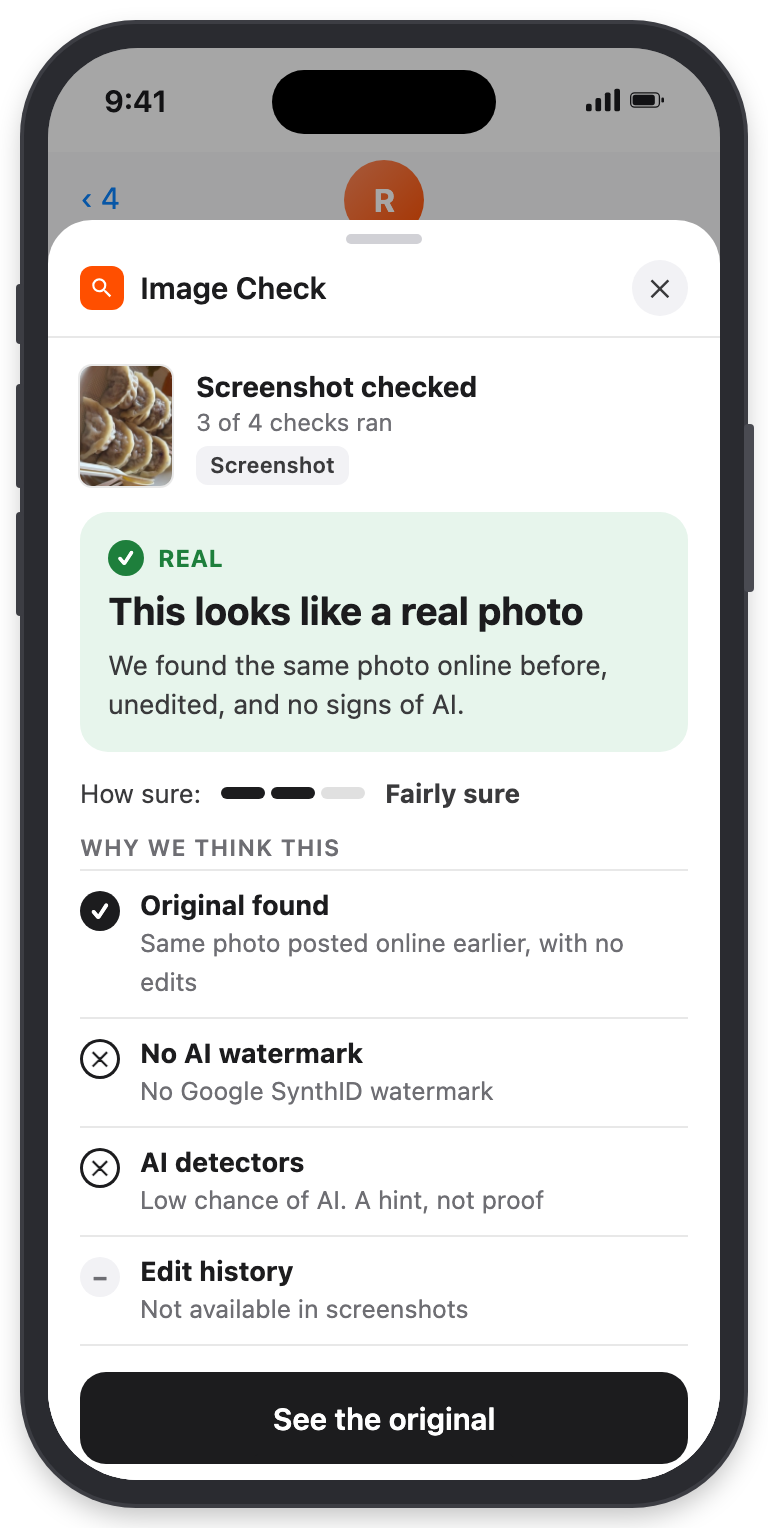
\includegraphics[height=4.95cm]{Screens/result_real.png}\par\vspace{0.06cm}\uilabel{real}{Real}\end{column}
    \begin{column}{0.235\linewidth}\centering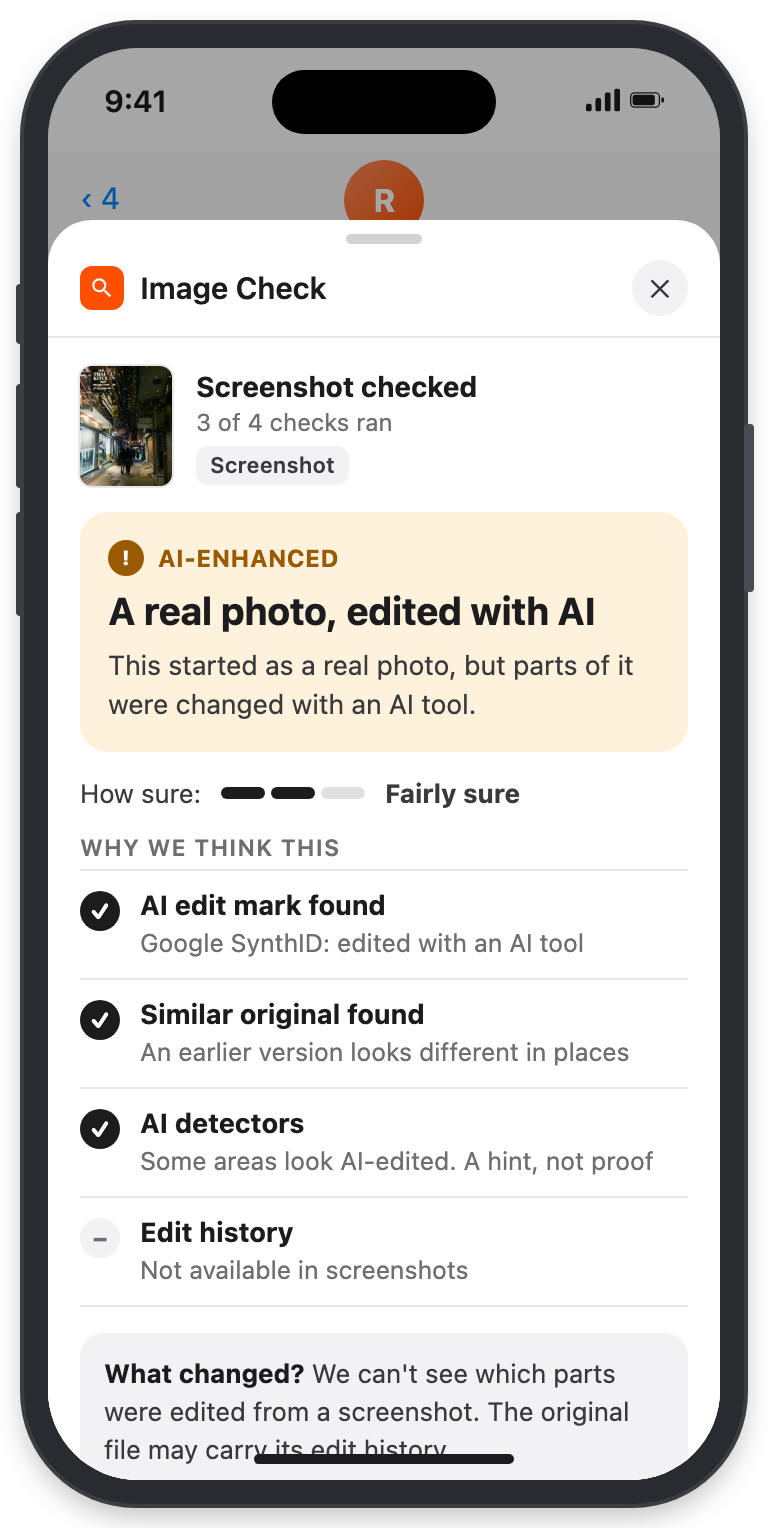
\includegraphics[height=4.95cm]{Screens/result_enhanced.png}\par\vspace{0.06cm}\uilabel{enh}{AI-enhanced}\end{column}
    \begin{column}{0.235\linewidth}\centering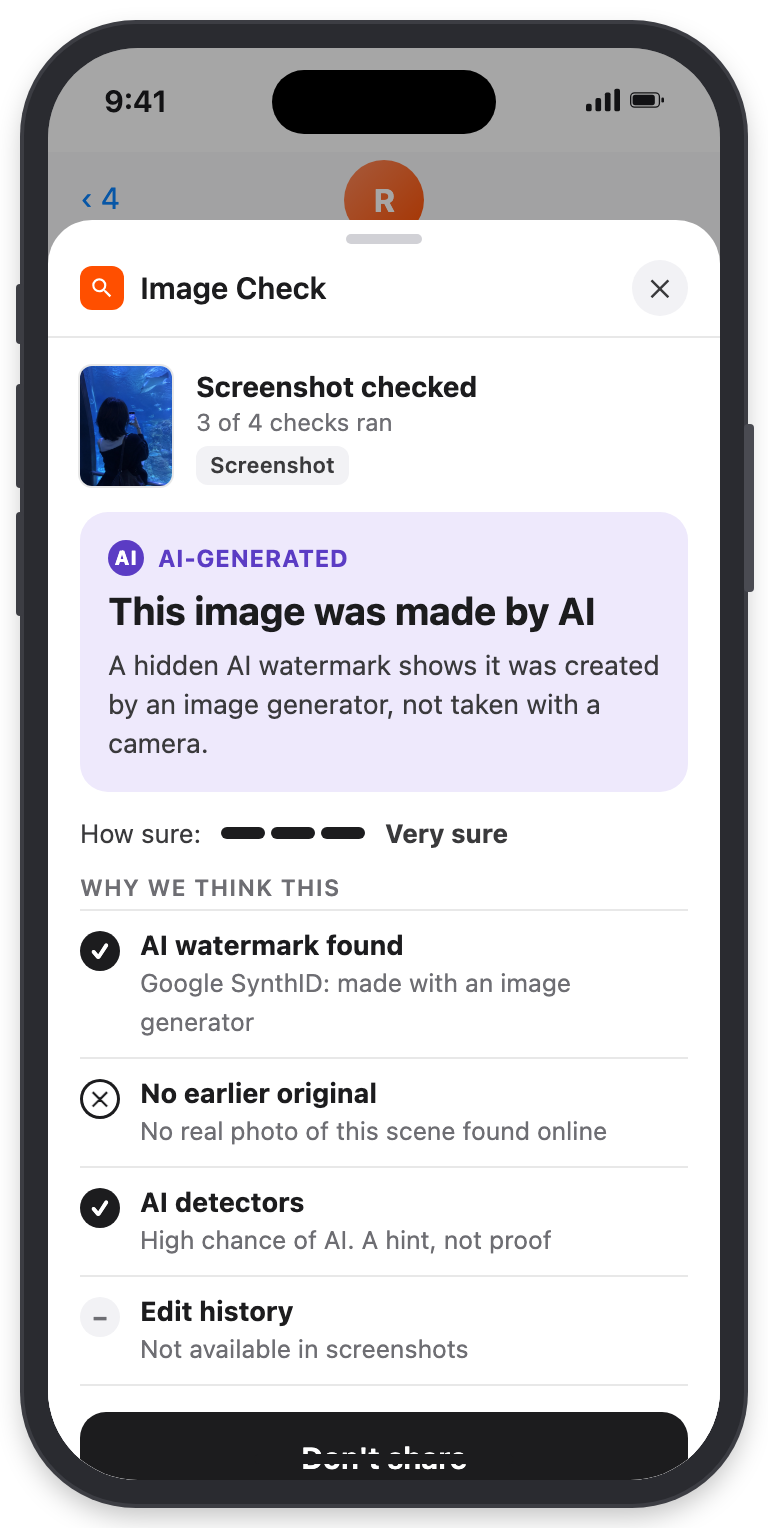
\includegraphics[height=4.95cm]{Screens/result_generated.png}\par\vspace{0.06cm}\uilabel{gen}{AI-generated}\end{column}
    \begin{column}{0.235\linewidth}\centering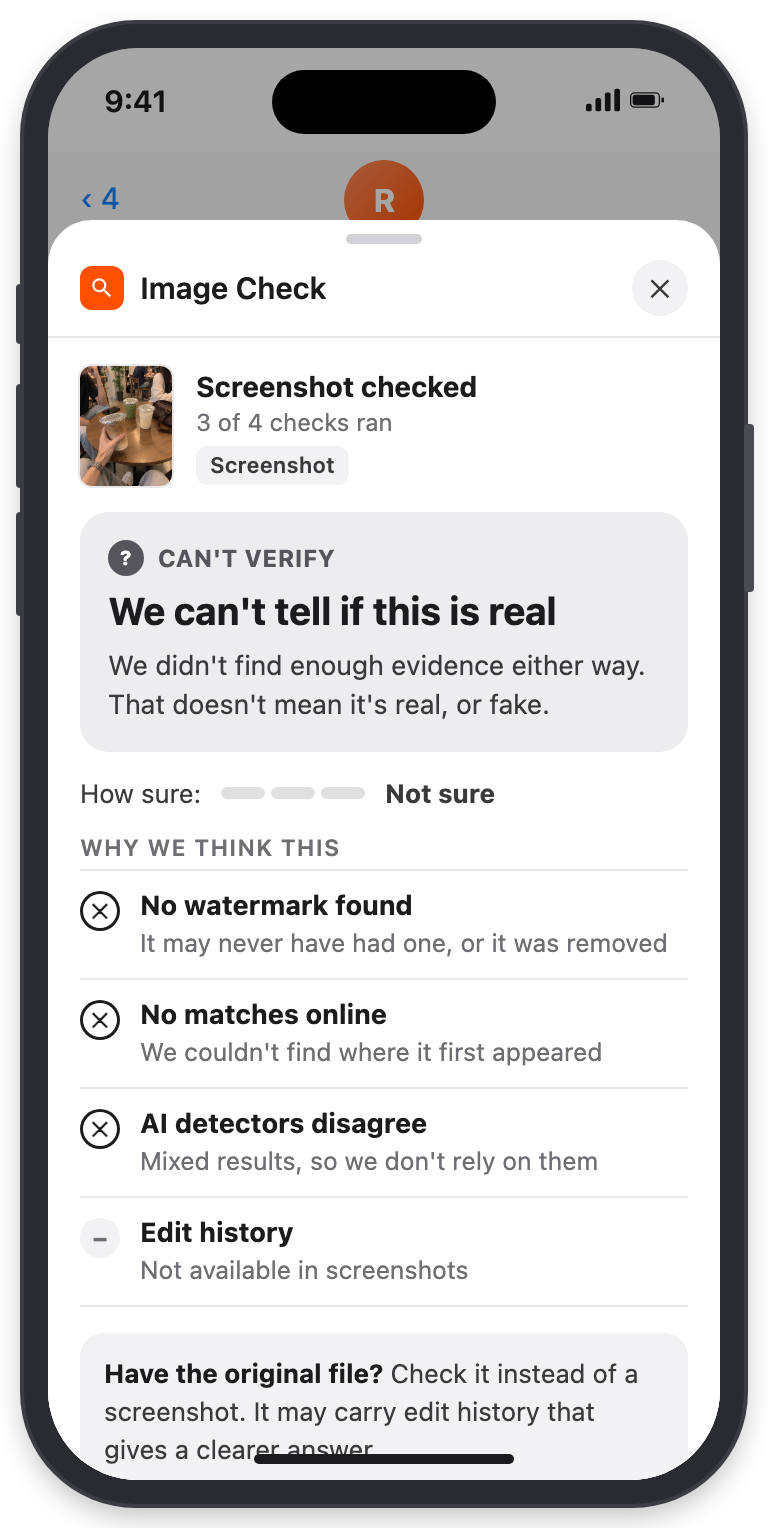
\includegraphics[height=4.95cm]{Screens/result_uncertain.png}\par\vspace{0.06cm}\uilabel{unk}{Can't verify}\end{column}
  \end{columns}
  \vspace{0.12cm}
  \meta{\color{mute}Each result has its own colour, icon and label, so it never relies on colour alone. Screenshots from the iPhone prototype.}
\end{frame}

\begin{frame}[plain, t]
  \chrome{4\quad Design}{TRUST \& EXPLAINABILITY}

  \slidehead{Trust \& explainability}
  \vspace{-0.2cm}
  \begin{columns}[T, onlytextwidth]
    \begin{column}{0.36\linewidth}
      \centering
      \begin{tikzpicture}
        \node[anchor=south west, inner sep=0] (img) at (0,0) {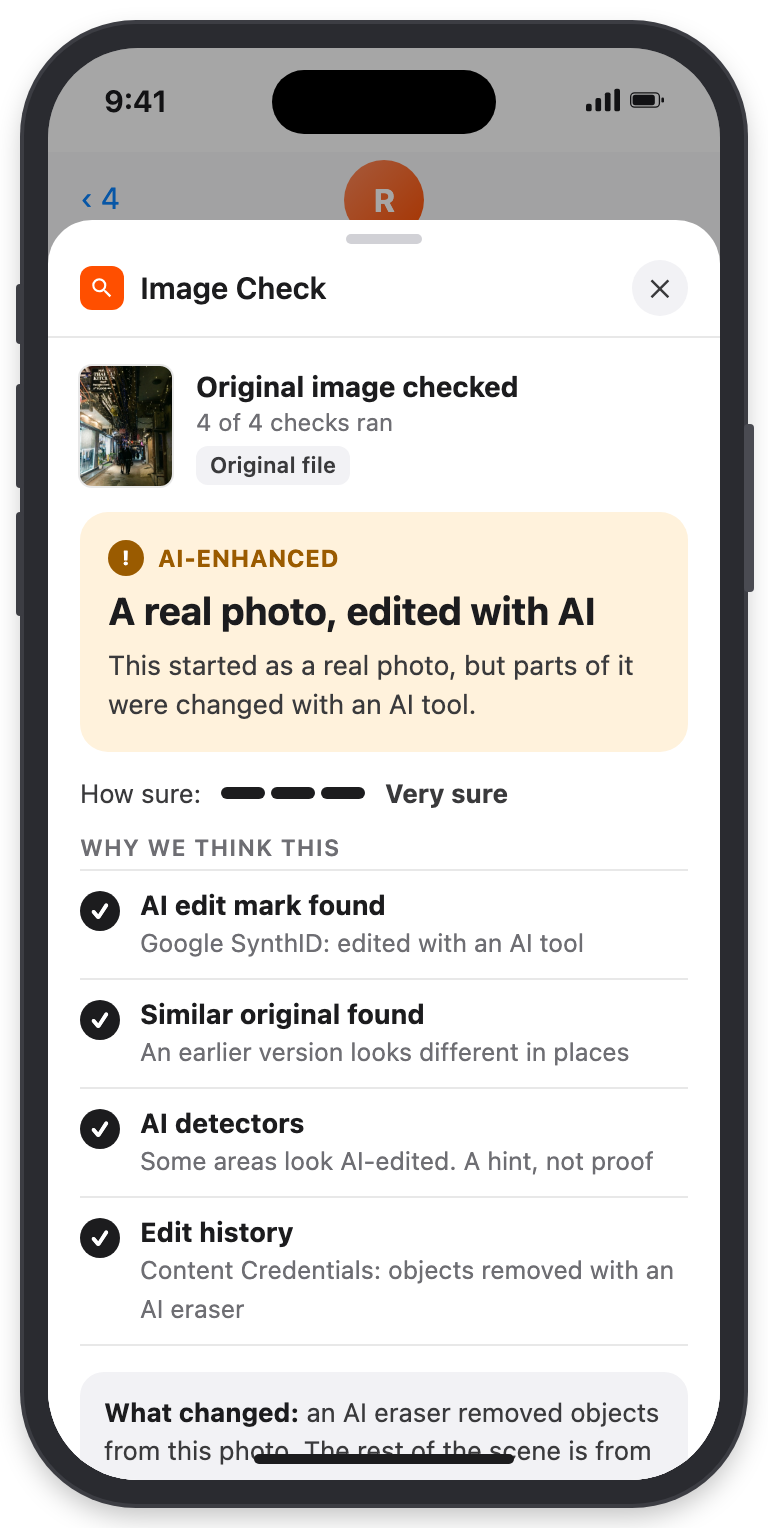
\includegraphics[height=5.75cm]{Screens/original_enhanced.png}};
        \begin{scope}[x={(img.south east)}, y={(img.north west)}]
          \foreach \n/\yy in {4/0.705, 1/0.585, 2/0.478, 3/0.32} {
            \node[circle, fill=accent, text=white, inner sep=0, minimum size=0.36cm, font=\fontsize{7.5pt}{8pt}\selectfont\bfseries] at (0.97, \yy) {\n};
          }
        \end{scope}
      \end{tikzpicture}
    \end{column}
    \begin{column}{0.6\linewidth}
      \trustrow{1}{The result, in plain words}{A label and one sentence. Never just ``fake''.}
      \trustrow{2}{How sure, in words}{A 3-step meter, no percentages. In my study, feeling sure was a weak guide.}
      \trustrow{3}{Why we think this}{Each check: found, not found, or not available.}
      \trustrow{4}{What was checked}{Screenshot or original file, and how many checks ran.}
      \trustrow{5}{You decide}{Next steps and ``I disagree''. Evidence, not a verdict.}
    \end{column}
  \end{columns}
\end{frame}

\begin{frame}[plain, t]
  \chrome{4\quad Design}{EDGE CASES}

  \slidehead{Key states \& edge cases}
  \begin{columns}[T, onlytextwidth]
    \begin{column}{0.31\linewidth}\edgecase{Mixed real + AI}{Labelled AI-enhanced. With edit history, highlight the changed areas.}{Planned for v2}\end{column}
    \begin{column}{0.31\linewidth}\edgecase{Not enough evidence}{``Can't verify'': not real, not fake. Suggest asking the sender.}{In prototype}\end{column}
    \begin{column}{0.31\linewidth}\edgecase{Conflicting signals}{Strongest evidence leads. Disagreements are shown and lower ``how sure''.}{Partly in prototype}\end{column}
  \end{columns}
  \vspace{0.25cm}
  \begin{columns}[T, onlytextwidth]
    \begin{column}{0.31\linewidth}\edgecase{Screenshot / reupload}{Edit history is lost. We say so and offer ``Check the original instead''.}{In prototype}\end{column}
    \begin{column}{0.31\linewidth}\edgecase{Wrong result}{Never a verdict. Detectors are ``a hint, not proof''.}{In prototype}\end{column}
    \begin{column}{0.31\linewidth}\edgecase{User disagrees}{``I disagree'' lets them pick their own label. The decision stays theirs.}{In prototype}\end{column}
  \end{columns}
\end{frame}

% =============================================================================
% 05 PROTOTYPE
% =============================================================================
\chapterslide{05}{Prototype}

\begin{frame}[plain, t]
  \chrome{5\quad Prototype}{CLICKABLE PROTOTYPE}

  \slidehead{Prototype}
  \begin{columns}[T, onlytextwidth]
    \begin{column}{0.48\linewidth}
      \colrule{Main way in: screenshot}
      \entry{1}{Take a screenshot {\color{mute}(phone: side button; laptop: drag a box)}}
      \entry{2}{Tap the thumbnail, or the pop-up}
      \entry{3}{Tap \textbf{Check for AI}}
      \entry{4}{Read the evidence and decide}
    \end{column}
    \begin{column}{0.48\linewidth}
      \colrule{Second way in: the original}
      \entry{Phone}{Share the image, then Image Check}
      \entry{Mac}{Drag the image onto the ``Drop to check'' pop-up}
      \vspace{0.05cm}
      \bodysm{{\color{mute}Checking the original adds its edit history: 4 of 4 checks instead of 3.}}
    \end{column}
  \end{columns}
  \vspace{0.3cm}
  \bodysm{\textbf{Detection is simulated; the focus is how results are explained.}}
  \bodysm{{\color{mute}Clickable prototype:} \href{https://claude.ai/artifact/66DqtYF2gPEZuyWrBWdS6N}{\color{accent}claude.ai/artifact/66DqtYF2gPEZuyWrBWdS6N}}
\end{frame}

% =============================================================================
% 06 MEASURE
% =============================================================================
\chapterslide{06}{Measure}

\begin{frame}[plain, t]
  \chrome{6\quad Measure}{SUCCESS METRICS \& NEXT STEPS}

  \slidehead{Success metrics \& next steps}
  \begin{columns}[T, onlytextwidth]
    \begin{column}{0.56\linewidth}
      \colrule{Success metrics}
      \entry{1}{\textbf{Check rate:} share of unsure images that get checked}
      \entry{2}{\textbf{Fewer risky shares:} AI-made or ``can't verify'' images forwarded after a check, vs before}
      \entry{3}{\textbf{Better judgement:} re-run my image task; beat the 58\% baseline, with confidence that matches accuracy}
      \entry{4}{\textbf{Understanding:} users can explain a result, e.g.\ ``can't verify'' isn't ``fake''}
      \vspace{0.04cm}
      \meta{\color{mute}Watched, not targeted: how often people tap ``I disagree''.}
    \end{column}
    \begin{column}{0.4\linewidth}
      \colrule{Next steps}
      \bul{Test if people find ``Check for AI''}
      \bul{Test with people aged 55+}
      \bul{Test the result wording}
      \bul{Highlight edited areas}
      \bul{Extend to video}
    \end{column}
  \end{columns}
\end{frame}

% =============================================================================
% TOOLS USED
% =============================================================================
\newcommand{\toolrow}[2]{%
  \par\vspace{0.07cm}{\color{hair}\hrule height 0.3pt}\vspace{0.12cm}
  \noindent\parbox[t]{5.4cm}{\fontsize{10pt}{13pt}\selectfont #1}%
  \hspace{0.3cm}\parbox[t]{\dimexpr\linewidth-5.7cm}{\fontsize{10pt}{13pt}\selectfont\leavevmode\color{mute}#2}\par\vspace{0.05cm}}
\begin{frame}[plain, t]
  \chrome{Tools used}{}

  \slidehead{Tools used}
  \toolrow{HTML, CSS, JavaScript}{Clickable prototypes (phone and laptop)}
  \toolrow{LaTeX (Beamer)}{Building this presentation}
  \toolrow{Claude (AI)}{Prototype code and LaTeX slides}
  \par\vspace{0.07cm}{\color{hair}\hrule height 0.3pt}
\end{frame}

% =============================================================================
% THANK YOU (orange)
% =============================================================================
{\setbeamercolor{background canvas}{bg=accent}
\begin{frame}[plain, t]
  \chromeorange{}{}
  \vfill
  {\fontsize{64pt}{64pt}\selectfont\tighttimes Thank you\par}
  \vspace{0.4cm}
  {\fontsize{10pt}{13pt}\selectfont Bulluraj Mutum \textperiodcentered{} M.Des (UX)\par}
  \vspace{0.9cm}
\end{frame}
}

\end{document}
